\chapter{基于$C_4$对称的声学拓扑晶体绝缘体的声传播与彩虹捕获研究}
\section{引言}
在上一章节中,我们讨论了亚波长尺度下,腔管结构的声学拓扑绝缘体的构造方法,并观察了其高阶拓扑态。一方面,对于如上一章节提到的无自旋并且时间反演不变的拓扑晶体绝缘体而言,其独特的拓扑态是由体极化来进行表征的。这种特性使得拓扑边界态在界面处有很强的鲁棒性。另一方面,我们的声学建模为在声学系统中实现这一类拓扑绝缘体提供了理论基础,我们可以根据理论模型里的相互作用,设计出对应尺寸的声学结构。如此一来,声学拓扑晶体绝缘体便自然而然地为利用特定的能量(也就是特定的频率)在结构的边界或者角落之处,以一种鲁棒的方式俘获波提供了一个极为理想的平台。

然而,尽管已经有大量细致入微的研究,无论是从理论层面还是实验层面,都确凿地证明了拓扑晶体绝缘体(TCIs)中存在着拓扑态,但是,像拓扑态的群速度这类与传播特性相关的内容,却鲜少被人们深入地探讨和研究。可实际上,这些传播特性在拓扑晶体绝缘体的实际应用当中,却是一个至关重要且无法回避的问题。

举个例子来说,利用拓扑态来实现彩虹俘获就是一个典型的应用场景。所谓的彩虹俘获,指的是将具有不同频率的波进行分离,并且让它们分别被俘获在不同的空间位置上。这种现象已经在多个领域的系统中被提出,比如在电磁波系统\cite{C41-1,C41-2,C41-3,C41-4,C41-5,C41-6,C41-7,C41-8,C41-9}、弹性波系统\cite{C42-1,C42-2,C42-3,C42-4,C42-5,C42-6}以及空气声系统\cite{C43-1,C43-2,C43-3,C43-4}中。在这些相关的研究工作里,研究人员们纷纷采用了各种各样的方法,其目的就是为了能够控制不同系统中波的色散关系,从而使得波能够在空间的不同位置上实现局域化。

不仅如此,一些近期的研究工作更是已经在拓扑态中成功地实现了彩虹俘获\cite{C44-1,C44-2,C44-3,C44-4,C44-5,C44-6}。在这些研究中,隙内模式能够在不减小体带隙的情况下被有效地减慢,而且体带隙依然能够受到强无序的良好保护。不过,令人遗憾的是,现有的这些方法通常都需要在体中设置额外的区域或者对晶格进行相应的变化。例如,在左边非平庸介质A和右边平庸的介质B构造一个界面,而拓扑边界态出现在中间的A和B界面之间,亦或是在平庸的环境中嵌入非平庸的介质,使得拓扑边界态出现在嵌入的非平庸介质周界。然而,在上一章节里,我们揭示了仅需要调控非平庸的声学结构以及边界条件,即可实现拓扑边界态。进一步,从实际应用的角度出发,我们还需要一种全新的方法,这种方法能够直接对边界处拓扑态的传播速度进行有效的控制。

因此,本章工作的目的是提出一种控制拓扑晶体绝缘体中不同频率下声波传播速度的方法,以实现声学彩虹俘获。基于二维(2D)Su-Schrieffer-Heeger(SSH)模型,我们严格证明了经典波系统的阻抗与紧束缚模型的跳跃项和在位项之间的对应关系,这表明,无需对体进行变形,通过仅仅调节超材料的表面阻抗,就可以精确且独立地控制边界态的群速度。这一特性天然为拓扑保护波俘获提供了一个新的思路,使得我们能利用边界态的鲁棒性的同时,也能大大减小结构的尺寸。由此我们通过实验展示了一个亚波长拓扑彩虹集中器的原型,其理论、仿真和实验结果显示这一结构可以时不同频率的声波停驻在拓扑绝缘体边界的不同位置。

本章主要内容如下:4.2节基于二维 SSH 声学拓扑晶体绝缘体,研究了体系的拓扑性质并深入探讨该绝缘体的特性以及在位势对其产生的影响等相关内容。4.3节着重阐述改变拓扑边界态的传播情况的相关原理,提出了改变表面阻抗从而改变拓扑边界态的群速度的方法。4.4节则围绕拓扑彩虹俘获的实验展开,详细介绍实现这一现象的具体过程、技术和相关要点。最后,4.5 节进行小结。

\section{二维SSH模型的拓扑性质}

\subsection{理论模型的哈密顿量}
\begin{figure}[h!]
    \centering
    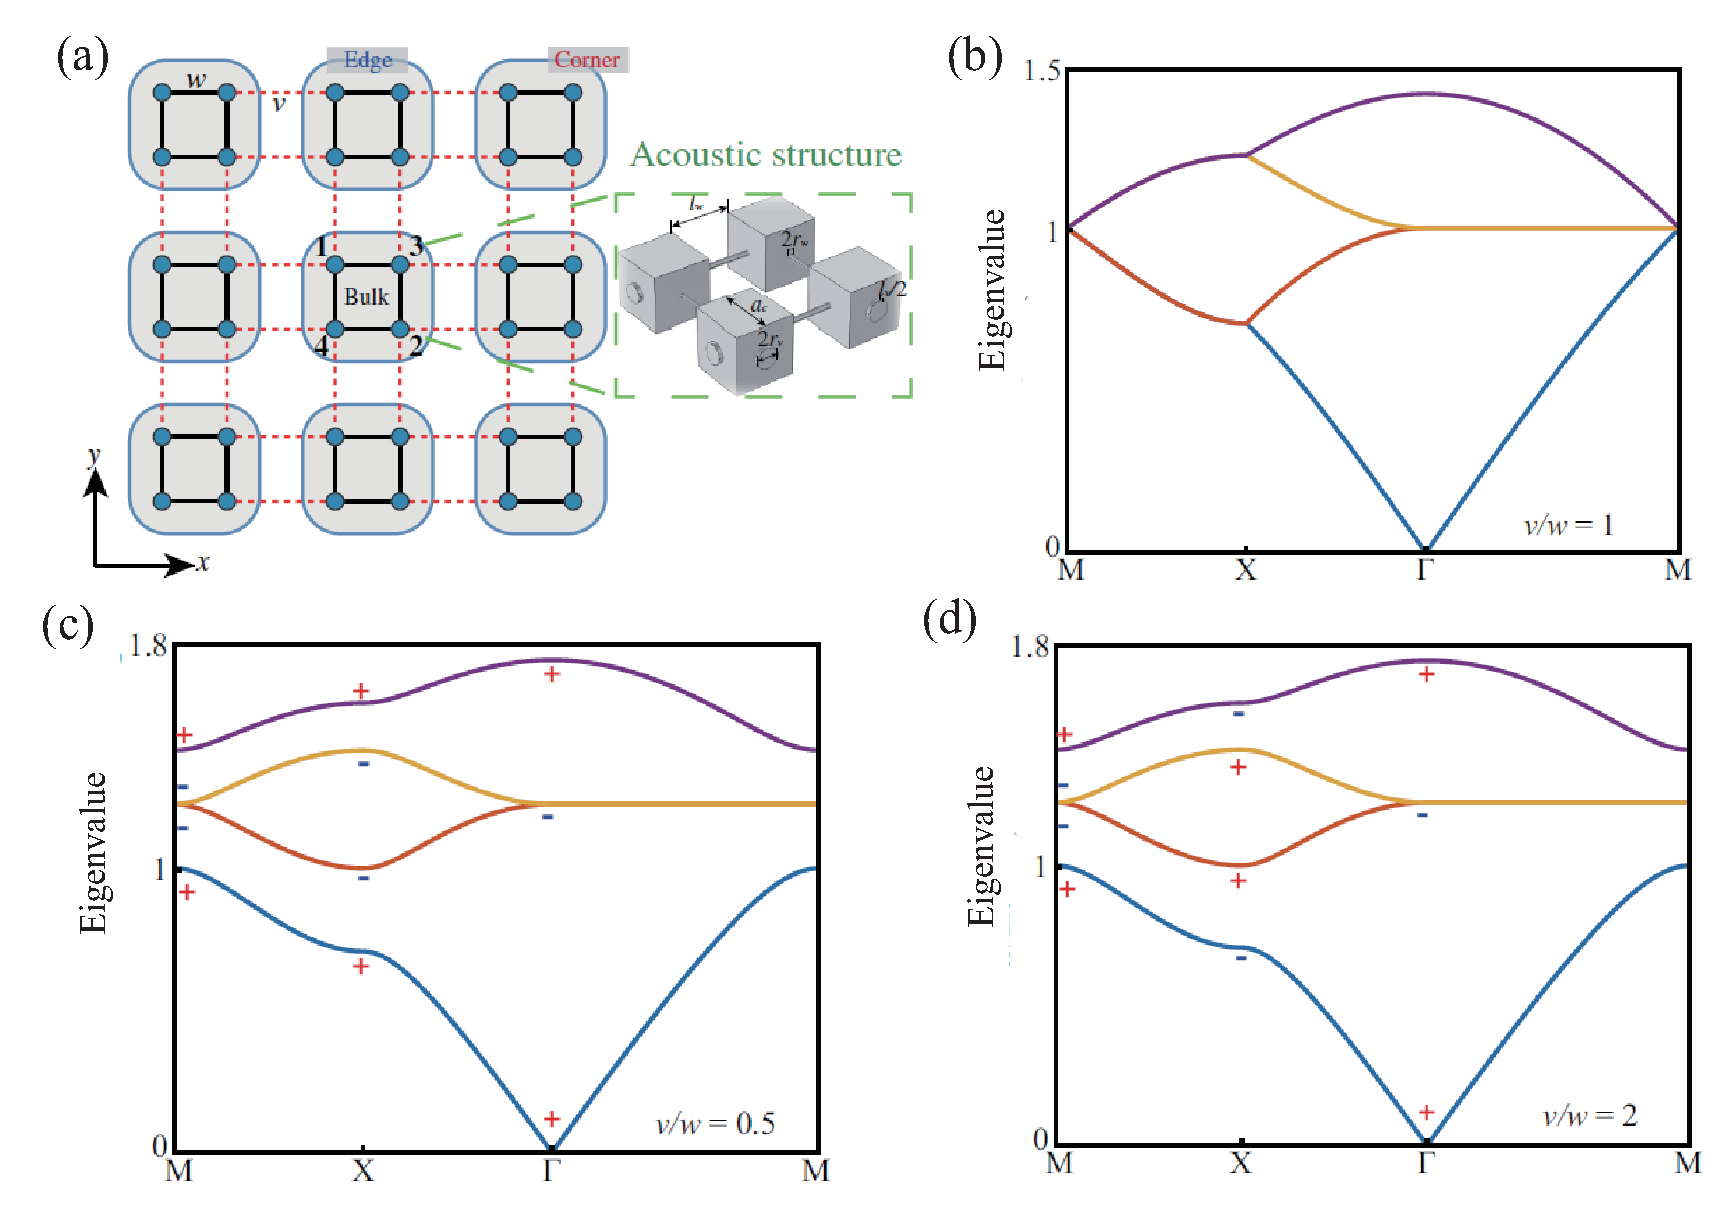
\includegraphics[width=1\textwidth]{images/fig4-1.eps} 
    \caption{(a) 二维SSH模型的示意图。(b-d)二维SSH模型的理论体能量带结构:(b)$v/w = 1$、(c)$v/w = 0.5$和(c)$v/w = 2$,“+/−”符号表示在高对称点处态的偶(+)奇(−)宇称。}
    \label{fig_4_1}
  \end{figure}  

在这部分,我们展示二维SSH紧束缚模型与声波系统之间对应关系的推导,并介绍其能带结构。首先,我们研究从如图\ref{fig_4_1}(a)所示的典型二维SSH模型开始,其中的结构满足$C_4$对称,$w$为胞内跳跃,$v$为胞间跳跃。用上一章节介绍的电子系统和声学系统类比思路,我们使用腔体模拟原子,用管道模拟格点跳跃,对应的声学腔管结构如图\ref{fig_4_1}(a)插图所示。其中,正方体腔体的边长位$a_c$,胞内和胞间导管的长度分别为$l_w$和$l_v$,半径分别为$r_w$和$r_v$。

在这里,我们定义在$(i,j)$晶格处的波函数(在声学系统里,可用声压作波函数)为$\Psi_{i,j} = [\psi_{i,j}^{(1)}, \psi_{i,j}^{(2)}, \psi_{i,j}^{(3)}, \psi_{i,j}^{(4)}]^T$,其中上标表示如文中图\ref{fig_4_1}(a)所标记的原子。通过上一章节展示的等效电路方法和基尔霍夫电流定律,可以得到方程
\begin{equation}
    \begin{aligned}
    -\frac{\psi_{(i,j)}^{(1)}}{Z_c} &= \frac{\psi_{(i,j)}^{(1)} - \psi_{(i,j)}^{(3)}}{Z_w} + \frac{\psi_{(i,j)}^{(1)} - \psi_{(i,j + 1)}^{(4)}}{Z_v} + \frac{\psi_{(i,j)}^{(1)} - \psi_{(i - 1,j)}^{(3)}}{Z_v} + \frac{\psi_{(i,j)}^{(1)} - \psi_{(i,j)}^{(4)}}{Z_w} \\
    -\frac{\psi_{(i,j)}^{(2)}}{Z_c} &= \frac{\psi_{(i,j)}^{(2)} - \psi_{(i,j + 1)}^{(4)}}{Z_v} + \frac{\psi_{(i,j)}^{(2)} - \psi_{(i + 1,j)}^{(3)}}{Z_w} + \frac{\psi_{(i,j)}^{(2)} - \psi_{(i,j)}^{(4)}}{Z_w} + \frac{\psi_{(i,j)}^{(2)} - \psi_{(i,j - 1)}^{(3)}}{Z_v} \\
    -\frac{\psi_{(i,j)}^{(3)}}{Z_c} &= \frac{\psi_{(i,j)}^{(3)} - \psi_{(i + 1,j)}^{(4)}}{Z_v} + \frac{\psi_{(i,j)}^{(3)} - \psi_{(i,j + 1)}^{(1)}}{Z_v} + \frac{\psi_{(i,j)}^{(3)} - \psi_{(i,j)}^{(1)}}{Z_w} + \frac{\psi_{(i,j)}^{(3)} - \psi_{(i,j)}^{(2)}}{Z_w} \\
    -\frac{\psi_{(i,j)}^{(4)}}{Z_c} &= \frac{\psi_{(i,j)}^{(4)} - \psi_{(i,j)}^{(2)}}{Z_w} + \frac{\psi_{(i,j)}^{(4)} - \psi_{(i,j)}^{(1)}}{Z_w} + \frac{\psi_{(i,j)}^{(4)} - \psi_{(i - 1,j)}^{(2)}}{Z_v} + \frac{\psi_{(i,j)}^{(4)} - \psi_{(i,j - 1)}^{(1)}}{Z_v}
    \end{aligned}
    \label{eq4-1}
\end{equation}

由于$Z_w = i\omega L_w$,$Z_v = i\omega L_v$且$Z_c = 1/i\omega C$,我们可以分别定义$w = -1/(L_wC)$和$v = -1/(L_vC)$。然后我们将所考虑的晶格标记为0,其左、下、右和上的最近邻晶格分别标记为$i = 1,2,3,4$。相应地,方程\ref{eq4-1}可重写为
\begin{equation}\label{eq4-2}
    \omega^2\Psi_0 = \hat{H}_0\Psi_0 + \sum_{i = 1}^{4} \hat{H}_i\Psi_i, 
\end{equation}
其中
\begin{equation}\label{eq4-3}
    \hat{H}_0 = 
    \begin{pmatrix}
    -2w - 2v & 0 & w & w \\
    0 & -2w - 2v & w & w \\
    w & w & -2w - 2v & 0 \\
    w & w & 0 & -2w - 2v
    \end{pmatrix}, 
\end{equation}
\begin{equation}\label{eq4-4}
    \hat{H}_1 = 
    \begin{pmatrix}
    0 & 0 & v & 0 \\
    0 & 0 & 0 & 0 \\
    0 & 0 & 0 & 0 \\
    0 & v & 0 & 0
    \end{pmatrix},
    \hat{H}_2 = 
    \begin{pmatrix}
    0 & 0 & 0 & 0 \\
    0 & 0 & v & 0 \\
    0 & 0 & 0 & 0 \\
    v & 0 & 0 & 0
    \end{pmatrix},
    \hat{H}_3 = 
    \begin{pmatrix}
    0 & 0 & 0 & 0 \\
    0 & 0 & 0 & 0 \\
    0 & 0 & 0 & v \\
    0 & 0 & 0 & 0
    \end{pmatrix},
    \hat{H}_4 = 
    \begin{pmatrix}
    0 & 0 & 0 & v \\
    0 & 0 & 0 & 0 \\
    0 & 0 & 0 & 0 \\
    0 & 0 & 0 & 0
    \end{pmatrix}, 
\end{equation}
进一步,通过应用傅里叶展开为
\begin{equation}\label{eq4-5}
    \Psi_0 = \sum_{k} \psi_k e^{i\vec{k} \cdot \vec{r}_0}
\end{equation}
\begin{equation}\label{eq4-6}
    \Psi_i = e^{i\vec{k} \cdot \vec{r}_i} \sum_{k} \psi_k e^{i\vec{k} \cdot \vec{r}_0},
\end{equation}
其中$i = 1,2,3,4$表示晶格0的左、下、右和上的最近邻晶格,$\vec{r}_i$是从晶格0指向它们的位置矢量。方程最终可以写成如下的形式
\begin{equation}\label{eq4-7}
    \omega_k^2 \psi_k = \hat{H}_k \psi_k,
\end{equation}
其中紧束缚模型的哈密顿量可表示为:
\begin{equation}
\hat{H}_k = 
\begin{pmatrix}
-2w - 2v & 0 & w + ve^{ik_x} & w + ve^{-ik_y} \\
0 & -2w - 2v & w + ve^{ik_y} & w + ve^{-ik_x} \\
w + ve^{-ik_x} & w + ve^{-ik_y} & -2w - 2v & 0 \\
w + ve^{ik_y} & w + ve^{ik_x} & 0 & -2w - 2v
\end{pmatrix}.
\label{eq4-8}
\end{equation}
相同的在位项不会影响体带的拓扑结构,并且该晶格仍可被视为保持手性对称性和\(C_4\)对称性,即:
\begin{equation}
[\Pi, \hat{H}_k + (2w + 2v)\mathbb{I}_{4\times4}] = 0, \quad [R_4, \hat{H}_k] = 0,
\label{eq4-9}
\end{equation}
其中\(\Pi\)和\(R_4\)分别是手性算符和旋转算符。

通过求解方程\ref{eq4-7},不同\(v/w\)的体晶格的能带结构分别如图\ref{fig_4_1}(b-d)所示。可以看出,在高对称点上,第一条和第二条能带间的带隙随着参数变化经过了打开,闭合再打开的过程,并且其态的宇称发了反转。具体而言,与二维Zak相相关的拓扑相变发生在\(w/v=1\)处。在此我们于图\ref{fig_4_1}(b)中展示了临界点处的能谱。在该临界点,四个能带在\(\Gamma\)点和\(X (Y)\)点相接触。由于子晶格对称性,\ref{fig_4_1}(c)图和(d)图能带反转后的能带结构相同。能带的拓扑性质由它们在高对称点处的宇称编码,这些宇称在图中标记为“\(\pm\)”。如图\ref{fig_4_1}所示,\(X (Y)\)点处最低\(s\)能带的宇称在能带反转后改变符号,这表明发生了拓扑相变。这种拓扑相变可由二维扩展Zak相来表征,其也是由以下表达式给出的波极化\cite{C45-1}:
\begin{equation}
    \mathbf{P}=\frac{1}{2\pi}\int dk_x dk_y \mathrm{Tr}[\mathbf{A}(k_x,k_y)]
    \label{eq4-10}
\end{equation}
其中\(\mathbf{A}=\langle\psi|i\partial_{\mathbf{k}}|\psi\rangle\)是Berry联络,积分是在第一布里渊区上进行的。反演对称性对\(\mathbf{P}\)的值施加了很强的约束,其由\(\Gamma\)点和\(X (Y)\)点处的宇称独立于规范确定,如下\cite{C45-2}:
\begin{equation}
    \mathcal{P}_i = \sum_{n}^{occ} q_i^n \bmod 2, \quad (-1)^{q_i^n} = \frac{\eta_n(X)}{\eta_n\Gamma}
    \label{eq4-11}
\end{equation}
其中\(\eta\)表示宇称,求和是对所有占据能带进行的,\(i\)代表\(x\)或\(y\)。由于\(C_4\)对称性,我们有\(\mathcal{P}_x = \mathcal{P}_y\)。基于式\Ref{eq4-11},能带反转后对于两个拓扑非平凡带隙可得到\(\mathbf{P}=(1/2,1/2)\),这表明在带隙内结构的边界和角落处可能存在局域的拓扑态。更关键的是,对于实际声学结构的边界晶格和角晶格(例如,图\ref{fig_4_1}(a)的上中晶格和上右晶格),由于内在的手性对称性破缺,有限结构哈密顿量中的相应部分可分别得到为:
\begin{equation}
\hat{H}_k^{edge} = 
\begin{pmatrix}
-2w - v & 0 & w & w \\
0 & -2w - 2v & w & w \\
w & w & -2w - v & 0 \\
w & w & 0 & -2w - 2v
\end{pmatrix},
\label{eq4-12}
\end{equation}
\begin{equation}
\hat{H}_k^{corner} = 
\begin{pmatrix}
-2w - v & 0 & w & w \\
0 & -2w - v & w & w \\
w & w & -2w & 0 \\
w & w & 0 & -2w - 2v
\end{pmatrix},
\label{eq4-13}
\end{equation}
因此,我们立即发现边界原子的不等在位势,实际上对应于广义手性对称性破缺\cite{i5},意味着在实际物理系统中边界局域态的能量移动。

\subsection{实际结构的拓扑边界态和角态}

\begin{figure}[h!]
    \centering
    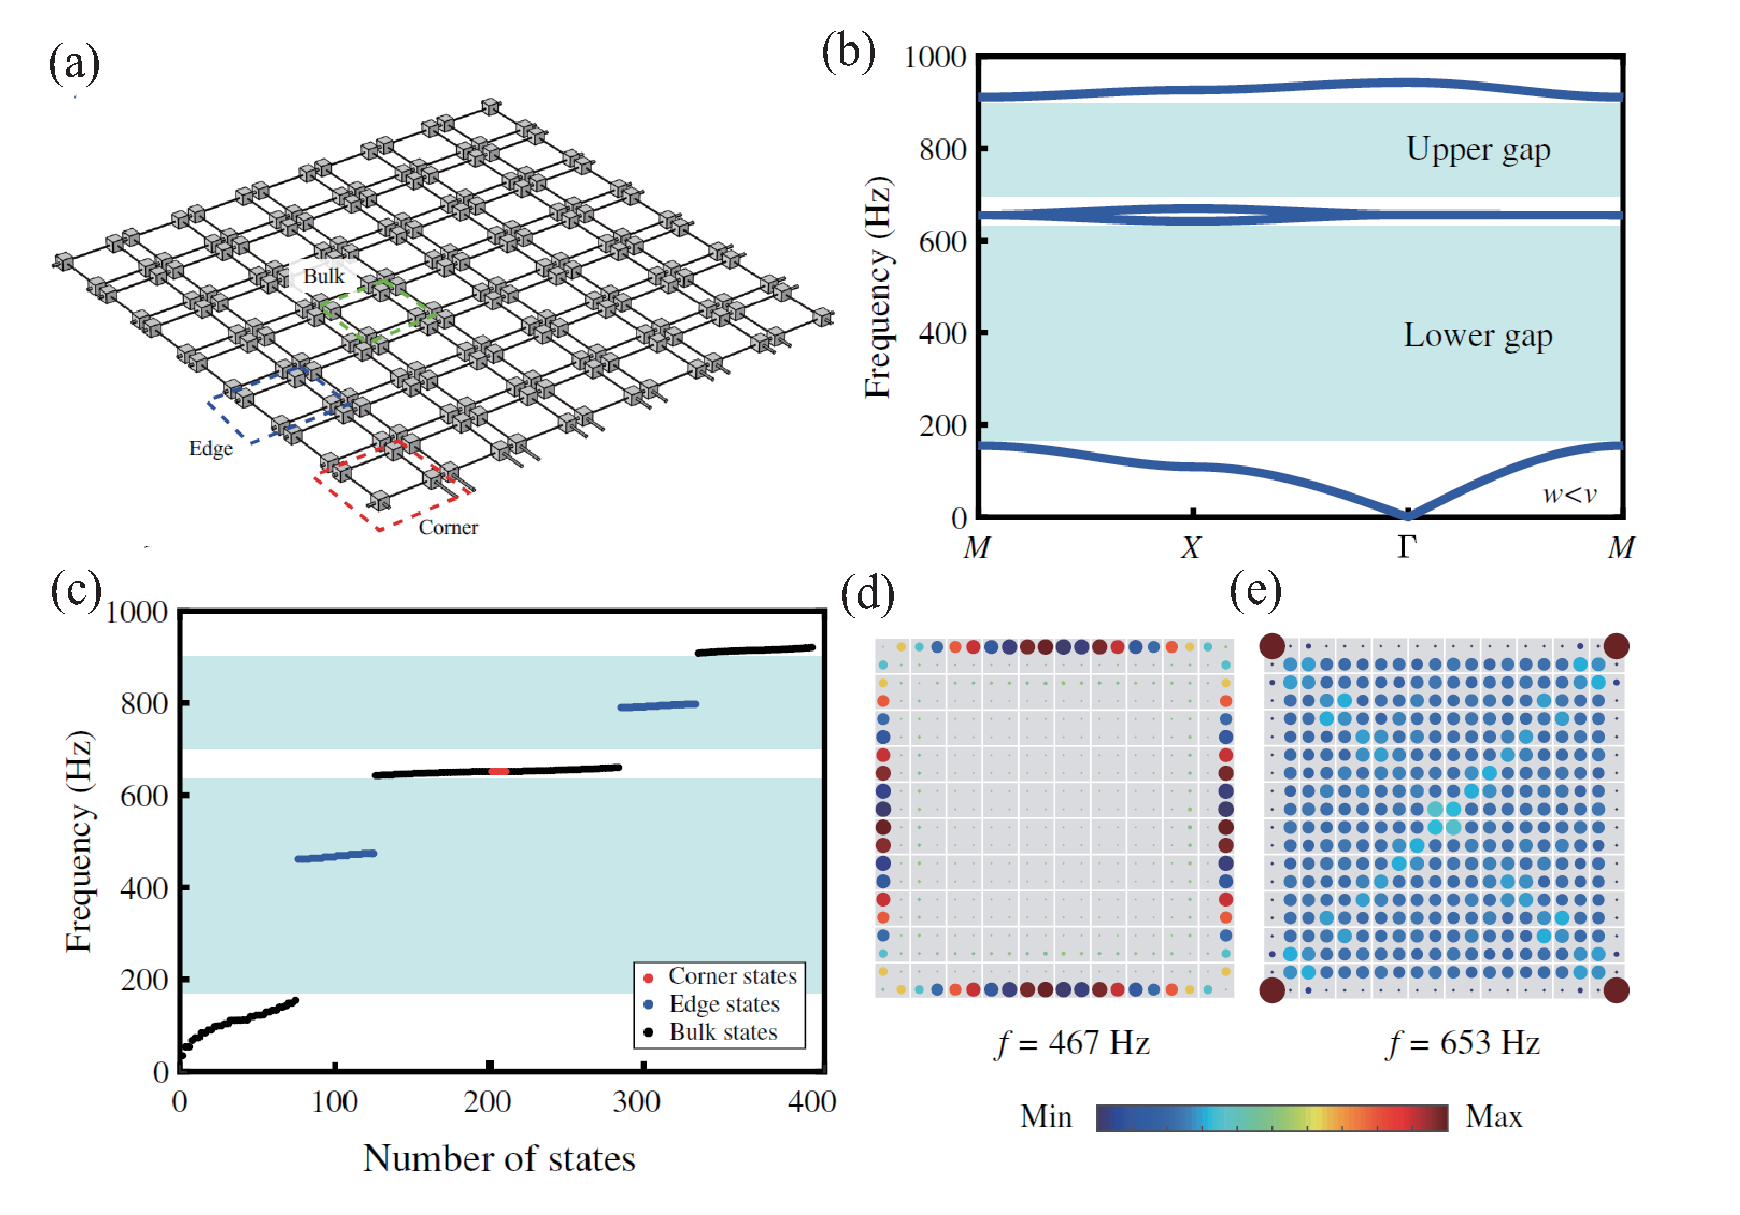
\includegraphics[width=1\textwidth]{images/fig4-2.eps} 
    \caption{(a)实际声学模型的示意图。(b)周期性结构的能谱。(c)有限结构的能谱。(d)在下带隙中孤立的边界局域态。(e)与体态简并的“零能”角局域态。}
    \label{fig_4_2}
  \end{figure}  

图\ref{fig_4_2}(b)展示了对于参数$a_c = 30$mm、$l_w = 120$mm、$l_v = 20$mm、$r_w = 1.5$mm和$r_v = 4$mm的能带结构。这里,连接腔体的晶内和晶间电感分别定义为$L_w$和$L_v$,而腔体的电容为$C$,可根据结构的几何参数获得。$\omega$是布洛赫波函数的角频率。对于体晶格,动量空间中本征值问题可写为方程\ref{eq4-7}。在当前情况下,跳跃项和阻抗之间的严格对应关系可直接得到为$w = -1/L_wC$和$v = -1/L_vC$(参见上一章节)。这里$w = -2.51\times 10^5$Hz$^2$且$v = -8.17\times 10^6$Hz$^2$。

由$C_4$对称性保护的第$n$个能带的高阶拓扑仍可由偶极矩$\mathcal{P}^{(n)} = (\mathcal{P}_x^{(n)}, \mathcal{P}_y^{(n)})$表征。此外,还可定义一个角诱导拓扑四极矩指数为\cite{C45-3}
\begin{equation}
    \mathcal{Q}_{xy} = \sum_{n = 1}^{\text{occ}} \mathcal{P}_x^{(n)} \mathcal{P}_y^{(n)}
    \label{eq4-14}
\end{equation}
对于此处有两个占据能带的情况,当$v > w$时,$\mathcal{P}_x^{(1)} = \mathcal{P}_y^{(1)} = \mathcal{Q}_{xy} = 0.5$,这表明在具有开放边界的有限结构的边界和角落处预计会出现拓扑边缘态和角落态,如图\ref{fig_4_2}(c)-(e)所示。

理论模型的一个内在考量是,即使在开放边界条件下,手性对称性也能完美保持,因此边界局域化模式预计会被固定到零能量(能隙中间);即使在许多实验研究中,在位势也总是被视为独立的。然而,如方程\ref{eq4-12}和\ref{eq4-13}所示,在位势与实际物理系统中的跳跃项强耦合。因此,对于有限结构,如果在边界晶格中没有严格的补偿,手性对称性的破坏将不可避免地导致在位势的偏移。例如,对于具有绝对硬壁边界条件的$C_4$对称声学系统或具有完美磁导体类似边界条件的光学系统,表面阻抗为$Z = \infty$,这使得边界晶格中的这些项为$\varepsilon^{\text{edge}} = -2w - v$,而角落晶格中原子的在位势为$\varepsilon^{\text{corner}} = -2w$。更重要的是,在相同条件下,最外层管道的长度直接决定它们的阻抗。从这个角度来看,我们可以改变相应位置管道的长度来改变位能,进而影响拓扑态的性质,例如拓扑边界态的传播速度或者是拓扑角态的频率,这将在下一节中详述。

\section{经典波系统中表面阻抗对拓扑态的影响}

在电子系统中,我们往往把真空看作是一种平庸介质,对非平庸的拓扑绝缘体,当存在某种空间对称性时其拓扑边界态出现在其表面,并且由于对称性保护拓扑角态出现在“零能”位置。但是,从上一小节可以看到,对实际的声学系统而言,表面阻抗的存在会影响非平庸结构的边界。虽然可观测的拓扑态通常被视作源自体拓扑,且被认为对于来自内部无序或平凡环境的干扰具备鲁棒性,然而在实际的物理系统里,若缺乏严格的边界补偿,手性对称性在本质上是被破坏的,这必然会致使边界在位势发生偏移,进而对拓扑态的出现产生影响。在本部分内容中,基于声学系统,我们深入且细致地分析了拓扑态存在的条件,并给出了这些态随着由表面阻抗表征的不同补偿所产生的能量偏移情况。 

\subsection{具有附加表面阻抗的一维SSH模型}

\begin{figure}[h!]
    \centering
    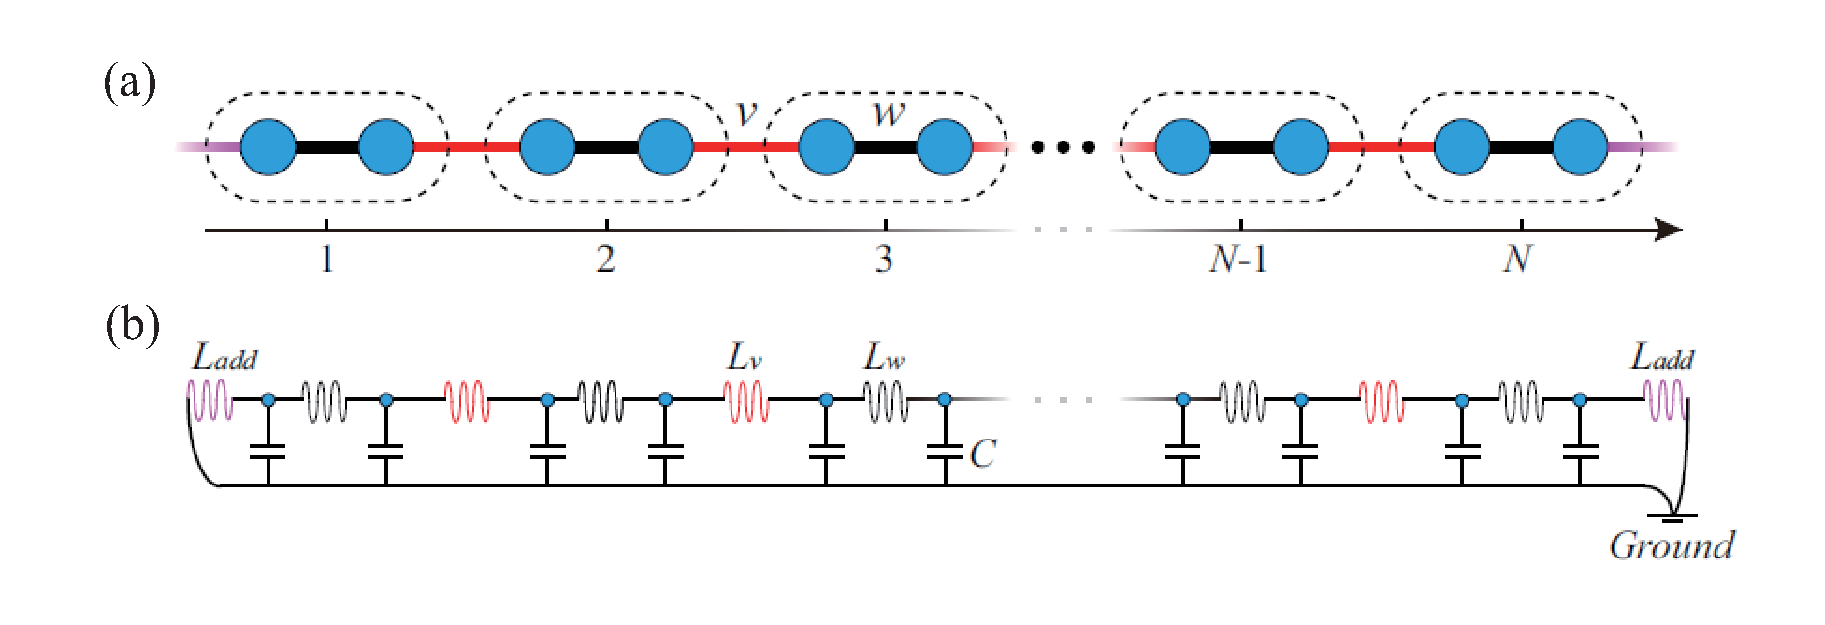
\includegraphics[width=1\textwidth]{images/fig4-3.eps} 
    \caption{(a)具有N个晶胞的一维SSH模型的示意图。(b)等效电路图。}
    \label{fig_4_3}
  \end{figure}  

在此,不失一般性,我们从具有\(N\)个单元的常规一维SSH模型开始,如图\ref{fig_4_3}(a)所示。我们分别将单元内和单元间阻抗定义为\(Z_{aa}\)和\(Z_{ab}\),原子的本征阻抗为\(Z_{c}\)。对于体中的第\(n\)个单元,原子\(a\)和\(b\)位置处的波函数可写为
\begin{equation}\label{eq4-15}
    \begin{split}
    -\frac{\psi_{n,a}}{Z_{c}} &= \frac{\psi_{n,a} - \psi_{n,b}}{Z_{w}} + \frac{\psi_{n,a} - \psi_{n - 1,b}}{Z_{v}},\\
    -\frac{\psi_{n,b}}{Z_{c}} &= \frac{\psi_{n,b} - \psi_{n,a}}{Z_{w}} + \frac{\psi_{n,b} - \psi_{n + 1,a}}{Z_{v}}.
    \end{split}
\end{equation}
因此,经典波系统中的单元内和单元间跳跃项可分别定义为\(w = \epsilon Z_{c} / Z_{aa}\)和\(v = \epsilon Z_{c} / Z_{ab}\),其中\(\epsilon\)与波函数\([\psi_{n,a},\psi_{n,b}]^T\)的频率\(\omega\)有关。把式\ref{eq4-15}重新整理,可重写为
\begin{equation}\label{eq4-16}
    \begin{split}
    (e + w + v)\psi_{n,a} &= w\psi_{n,b} + w\psi_{n - 1,b},\\
    (e + w + v)\psi_{n,b} &= w\psi_{n,a} + w\psi_{n + 1,a}.
    \end{split}
\end{equation}
对于边界单元,即第一个单元和第\(N\)个单元,我们在末端的原子上施加一个额外阻抗\(Z_{add}=Z_{v}+Z\),这在实际声学结构中非常常见,因为实际结构边界处的表面阻抗总是需要仔细考量的。相应单元中的波函数则可表示为
\begin{equation}\label{eq4-17}
    \begin{split}
    (\epsilon + w + \Delta_0)\psi_{1,a} &= w\psi_{1,b},\\
    (\epsilon + w + \Delta_0)\psi_{N,b} &= w\psi_{N,a}.
    \end{split}
    \end{equation}
其中\(\Delta_0 = \epsilon Z_{c} / Z_{add} = vZ_{v} / (Z_{v} + Z)\)。值得注意的是,在实际物理系统中,原子可由纯电容\(C\)表征,原子间的相互作用可由纯电感\(L_{\alpha}(\alpha = w,v)\)表征。因此,我们得到关系\(Z_{c} = 1 / i\omega C\)和\(Z_{\alpha} = i\omega L_{\alpha}\)。此外,从\(\Delta_0\)的定义可以容易地得出\(Z = i\omega L\)应归因于纯电感[如图\ref{fig_4_3}(b)所示]。这是由于腔管结构的表面往往是控制导管来控制表面阻抗,否则实际结构可能无法和电子系统中线性的本征值问题很好地对应上,而这在本工作中未被考虑。结果,式\ref{eq4-17}最终可重写为
\begin{equation}\label{eq4-18}
    \begin{split}
    (\epsilon + w + v + \Delta)\psi_{1,a} &= w\psi_{1,b},\\
    (\epsilon + w + v + \Delta)\psi_{N,b} &= w\psi_{N,a}.
    \end{split}
\end{equation}
值得一提的是,由于在实际结构中\(L \in [0,\infty]\),我们得到\(\Delta \in [-v,0]\)。

\subsection{平庸体态和拓扑态的解析解}

实际上,系统的哈密顿量可直接从式\ref{eq4-15}和\ref{eq4-16}导出。然而,这种方法难以区分平庸体态和拓扑态。在此,我们使用一种直接方法,通过获得解析解来讨论拓扑态的存在。我们使用第\(n\)个单元中波函数的通解为\cite{i5}
\begin{equation}\label{eq4-19}
    \begin{split}
        \psi_{n,a}=A_{1}\gamma^{n}+A_{2}\gamma^{-n},\\
        \psi_{n,b}=B_{1}\gamma^{n}+B_{2}\gamma^{-n},
    \end{split}
\end{equation}
其中\(\{A_{1},A_{2},B_{1},B_{2}\}\)是正向和反向平面波的幅值系数。因此,若\(\gamma=\xi e^{i\theta}(\theta\in[-\pi,\pi])\)为虚数则表示体中具有周期性场分布的平凡态,而\(\gamma\)为实数(\(\gamma\neq\pm1\))表示从边界向体中指数衰减的拓扑态。我们将通解\ref{eq4-19}代入式\ref{eq4-16},得到
\begin{equation}\label{eq4-20}
    \begin{split}
        {P}_{1}\gamma^{n}-\mathcal{P}_{2}\gamma^{-n}=0,\\
        {P}_{3}\gamma^{n}-\mathcal{P}_{4}\gamma^{-n}=0,
    \end{split}
\end{equation}
其中
\begin{equation}\label{eq4-21}
    \begin{split}
        {P}_{1}=\epsilon'A_{1}-wB_{1}-vB_{1}\gamma^{-1},\\
        {P}_{2}=\epsilon'A_{2}-wB_{2}-vB_{2}\gamma,\\
        {P}_{3}=\epsilon'B_{1}-wA_{1}-vA_{1}\gamma^{-1},\\
        {P}_{4}=\epsilon'B_{2}-wA_{2}-vA_{2}\gamma^{-1},
    \end{split}
\end{equation}
其中\(\epsilon' = w + v + \epsilon\)。然后我们可以得到\({P}_{i}=0\ (i = 1,2,3,4)\)的关系,以满足每个体单元中的波函数。结果,我们得到
\begin{equation}\label{eq4-22}
    \epsilon'\begin{bmatrix}B_{1}\\A_{1}\\A_{2}\\B_{2}\end{bmatrix}=\begin{bmatrix}\mathcal{D}_{2\times2}&\mathcal{O}\\\mathcal{O}&\mathcal{D}_{2\times2}\end{bmatrix}\begin{bmatrix}B_{1}\\A_{1}\\A_{2}\\B_{2}\end{bmatrix}
\end{equation}
其中
\begin{equation}\label{eq4-23}
    \mathcal{D}_{2\times2}=\begin{bmatrix}0&w + v\gamma\\w + v\gamma^{-1}&0\end{bmatrix},
\end{equation}
对于矩阵\(\mathcal{D}_{2\times2}\),存在两个不相等的非零特征值,即
\begin{equation}\label{eq4-24}
    \begin{split}
        \epsilon_{1}' = -\sqrt{(w + v\gamma)(w + v\gamma^{-1})},\\
        \epsilon_{2}' = -\epsilon_{1}'
    \end{split}
\end{equation}
因此,对于式\ref{eq4-22},应当有两对双重特征值,分别对应两对独立的特征向量。然后我们将与\(\mathcal{D}_{2\times2}\)的特征值\(\epsilon'\)对应的特征向量定义为\(\mathbf{u} = [u_{1}\ u_{2}]^{T}\),式\ref{eq4-22}的特征向量空间最终得到
\begin{equation}\label{eq4-25}
    \begin{bmatrix}B_{1}\\A_{1}\\A_{2}\\B_{2}\end{bmatrix}=\alpha\begin{bmatrix}u_{1}\\u_{2}\\0\\0\end{bmatrix}+\beta\begin{bmatrix}0\\0\\u_{1}\\u_{2}\end{bmatrix}=\begin{bmatrix}\alpha u_{1}\\\alpha u_{2}\\\beta u_{1}\\\beta u_{2}\end{bmatrix},
\end{equation}
其中\(\alpha\)和\(\beta\)是任意系数。因此,式S18可重写为
\begin{equation}\label{eq4-26}
    \begin{split}
        \psi_{n,a}=\alpha u_{2}\gamma^{n}+\beta u_{1}\gamma^{-n},\\
        \psi_{n,b}=\alpha u_{1}\gamma^{n}+\beta u_{2}\gamma^{-n},
    \end{split}
\end{equation}
为了方便讨论,这里特征向量的基选择为\(u_{1}=w + v\gamma\)和\(u_{2}=\epsilon'\)。将式\ref{eq4-26}代入式\ref{eq4-20},我们得到
\begin{equation}\label{eq4-27}
    \mathcal{F}\begin{bmatrix}x\\y\end{bmatrix}=\begin{bmatrix}0\\0\end{bmatrix},
\end{equation}
其中
\begin{equation}\label{eq4-28}
    \mathcal{F}=\begin{bmatrix}\{(\epsilon'+\Delta)u_{2}-wu_{1}\}\gamma&\{(\epsilon'+\Delta)u_{1}-wu_{2}\}\gamma^{-1}\\\{(\epsilon'+\Delta)u_{1}-wu_{2}\}\gamma^{N}&\{(\epsilon'+\Delta)u_{2}-wu_{1}\}\gamma^{-N}\end{bmatrix},
\end{equation}
方程存在的非平凡解要求\(\mathrm{det}(\mathcal{F}) = 0\),所以得到
\begin{equation}\label{eq4-29}
    w^{2}F(\gamma)=\{(\epsilon'+\Delta)u_{2}-wu_{1}\}^{2}\gamma^{-N + 1}-\{(\epsilon'+\Delta)u_{1}-wu_{2}\}^{2}\gamma^{N - 1}=0,
\end{equation}
将式\ref{eq4-24}代入式S\ref{eq4-29},\(\gamma\)可以很好地确定,并且由于\(F(\gamma)=F(-\gamma)\)的性质,很明显该方程有\(N\)对相反的根。同时,系数\([\alpha\ \beta]^{T}\)可定义为
\begin{equation}\label{eq4-30}
    \begin{bmatrix}\alpha\\\beta\end{bmatrix}=\begin{bmatrix}-\{(\epsilon'+\Delta)u_{2}+wu_{1}\}\gamma^{-1}\\\{(\epsilon'+\Delta)u_{1}-wu_{2}\}\gamma\end{bmatrix},
\end{equation}
结果,所有系数\(\{\alpha,\beta,\gamma\}\)都可以在\(\Delta\)定义的情况下直接得到。

\subsection{经典波系统的限制条件}

我们注意到\(\epsilon_{1}'\)和\(\epsilon_{2}'\)都可以确定\(\gamma\)的解析解。然而,在实际物理系统中,\(\Delta\in[-v,0]\)这一事实表明只有\(\epsilon_{1}'\)具有明确的物理意义,而\(\epsilon_{2}'\)在本工作中不做讨论。另一方面,我们认为\(\gamma=\pm1\)是一对不满足式\ref{eq4-24}的异常解。然而,这两种情况可以从式\ref{eq4-16}和\ref{eq4-18}中精确求解。

(i)\(\gamma = 1\)情况。我们假设\(\psi_{n,a}=A\)且\(\psi_{n,b}=B\),分别将这些函数代入式\ref{eq4-16},然后我们立即得到\(\epsilon'=\pm(w + v)\)且\(A/B=\pm1\)。此外,式\ref{eq4-18}得出
\begin{equation}\label{eq4-31}
    \epsilon' = w + v, \Delta = -v;
\end{equation}

(ii)\(\gamma = -1\)情况。我们假设\(\psi_{n,a}=(-1)^{n}A\)且\(\psi_{n,b}=(-1)^{n}B\),分别将这些函数代入式S13,然后我们得到\(\epsilon'=\pm(w - v)\)且\(A/B=\pm1\)。此外,式\ref{eq4-18}得出
\begin{equation}\label{eq4-32}
    \epsilon' = -w + v, \Delta = -v;
\end{equation}

如上所述,\(\gamma=\pm1\)是\(Z=\infty\)条件下的一对解。此外,对于体态\(\gamma=\xi e^{i\theta}\),很容易证明\(\xi^{2}=1\)。

\subsection{拓扑态存在的边界条件}

\begin{figure}[h!]
    \centering
    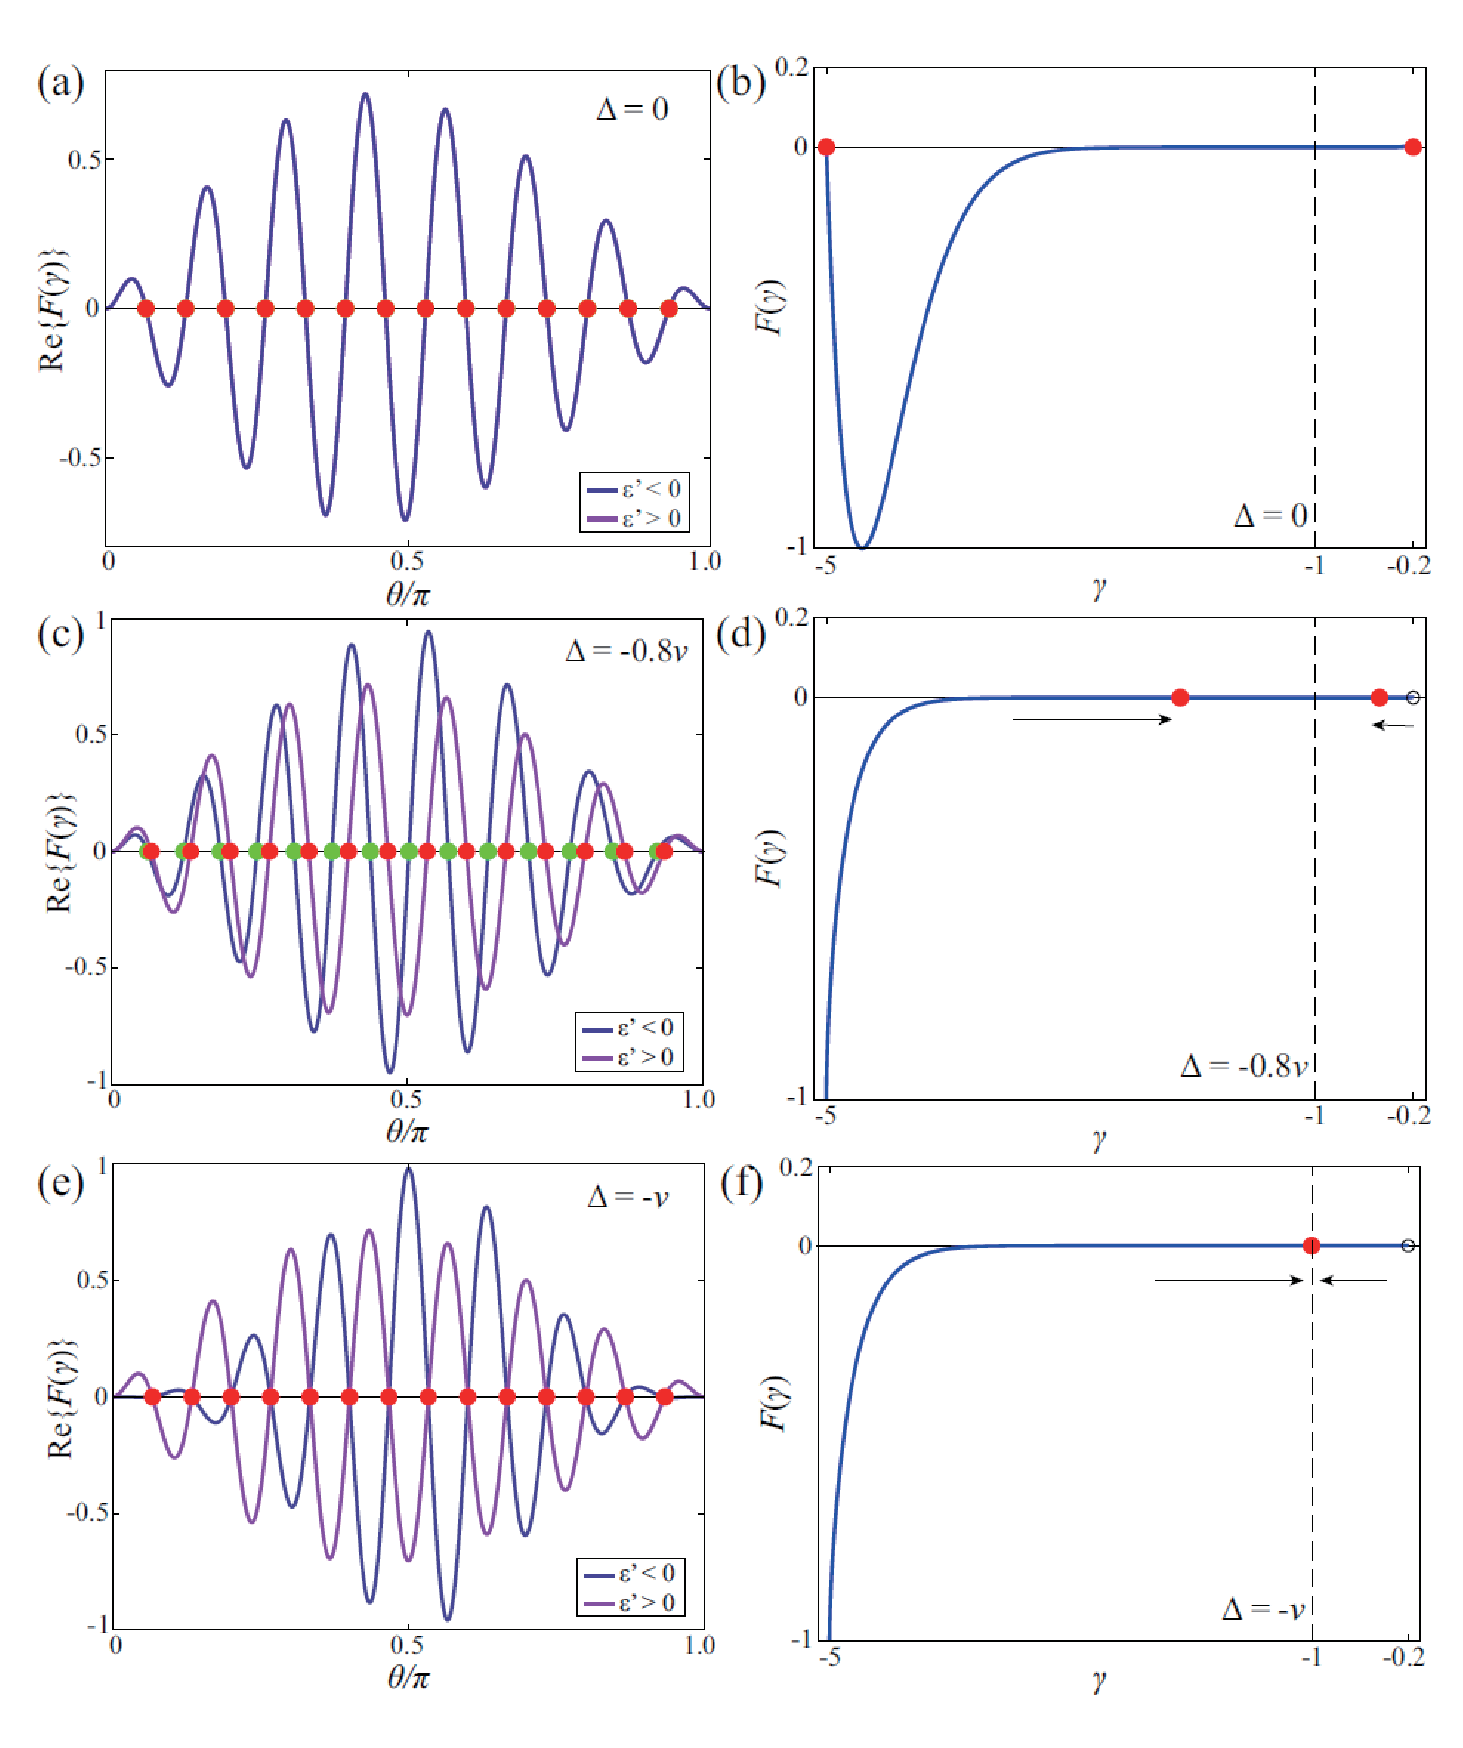
\includegraphics[width=1\textwidth]{images/fig4-4.eps} 
    \caption{当(a)$\Delta = 0$(声学绝对软壁边界条件)、(c)$\Delta = -0.8v$以及(e)$\Delta = -v$(声学绝对硬壁边界条件)时,具有不同复$\gamma$的无量纲$F(\gamma)$,分别如所示。当(b)$\Delta = 0$、(d)$\Delta = -0.8v$以及(f)$\Delta = -v$时,具有不同实$\gamma$的$F(\gamma)$,分别如所示。(d)和(f)中的箭头指示了具有不同$\Delta$时$\gamma$的移动方向。}
    \label{fig_4_4}
\end{figure} 

\begin{figure}[h!]
    \centering
    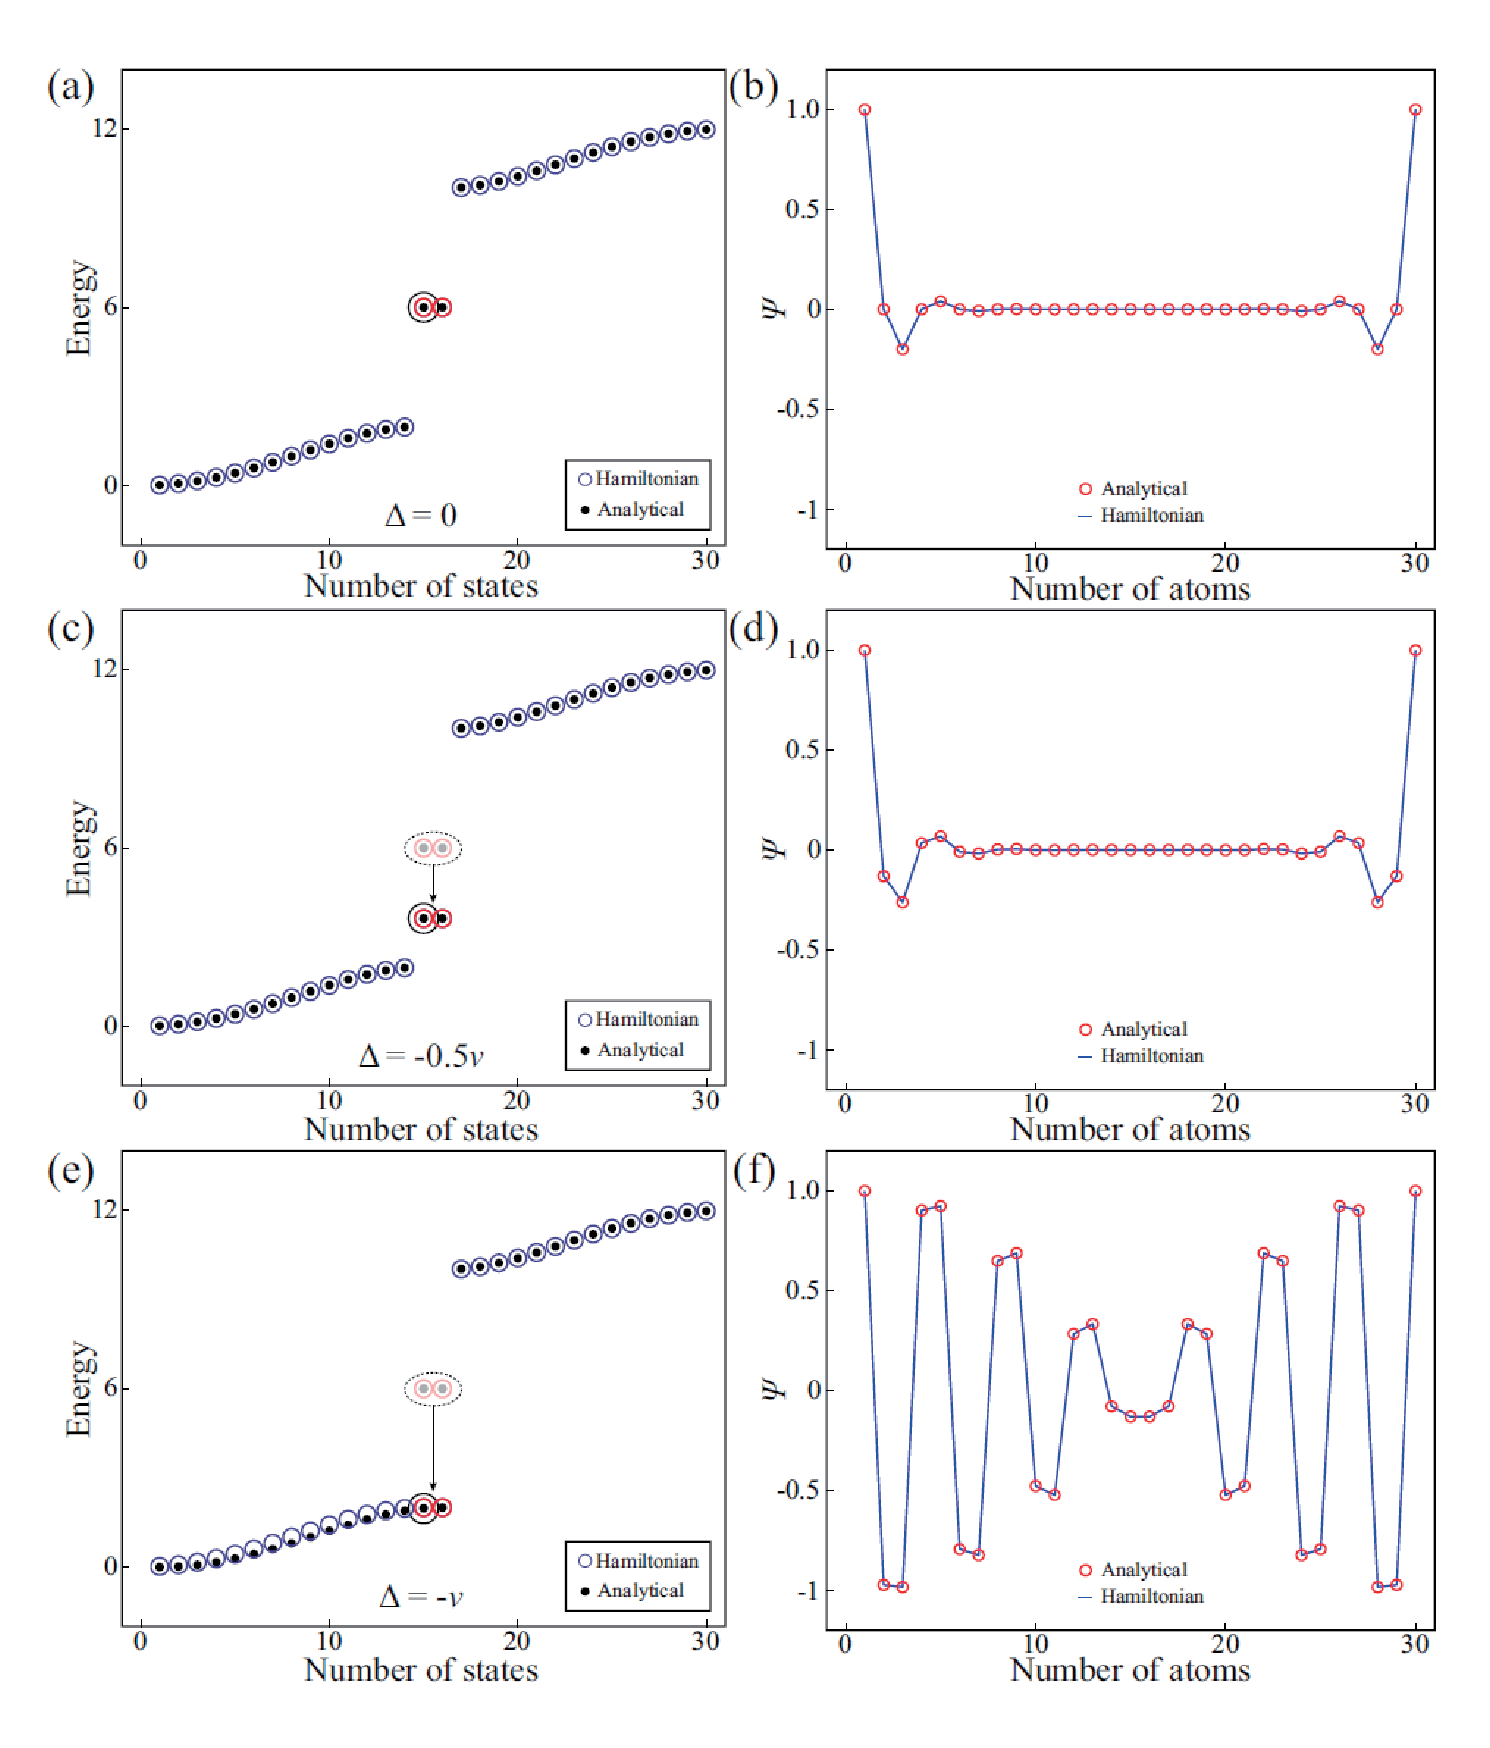
\includegraphics[width=1\textwidth]{images/fig4-5.eps} 
    \caption{当(a)$\Delta = 0$(声学绝对软壁边界条件)、(c)$\Delta = -0.5v$以及(e)$\Delta = -v$(声学绝对硬壁边界条件)时,由哈密顿量(蓝色圆圈)和解析方法(黑色点)得到的能谱,分别如所示。(b)、(d)、(f)分别为(a)、(c)和(e)中拓扑态(用黑色圆圈圈出)的相应场分布。能量单位为$Hz^2$,$\Psi$是无量纲的。}
    \label{fig_4_5}
\end{figure} 

如上所述,在实际物理系统中,\(\Delta\)的范围是从\(-v\)到\(0\)。值得注意的是,两个极端条件,即\(\Delta = -v\)和\(\Delta = 0\),分别对应于表面阻抗\(Z\)为\(\infty\)和\(0\)。例如,在经典波系统中,\(Z=\infty\)表示光学系统中类似完美磁导体的边界或声学系统中绝对硬壁边界,而\(Z = 0\)表示光学系统中类似完美电导体的边界或声学系统中绝对软壁边界。在下文中,我们基于声学系统讨论边界条件。

(i)绝对硬壁边界条件(\(Z=\infty\))——将\(\Delta = -v\)代入式\ref{eq4-29}得出
\begin{equation}
    \gamma^{2N}=1,
\end{equation}
然后我们得到解为\(\gamma = e^{i\frac{2\pi}{N}i}\),其中\(i = 1,2,\cdots,N - 1\)。再加上根\(\gamma = 1\),我们最终得到所有\(N\)个正根,值得注意的是所有这些根都表示体态。进一步,解\(\gamma=\pm1\)实际上可以被视为与体态混合的简并拓扑态(如下所述)。

(ii)绝对软壁边界条件(\(Z = 0\))——在这种情况下,我们将\(\Delta = 0\)代入式\ref{eq4-29},得到
\begin{equation}\label{eq4-34}
(w + v\gamma^{-1})\gamma^{N + 1}-(w + v\gamma)\gamma^{-N - 1}=0,
\end{equation}
式\ref{eq4-34}有\(2N + 2\)个根。除了如上所述的\(\gamma=\pm1\),我们最终得到所有\(2N\)个根。注意,当\(N\rightarrow\infty\)时,只有当\(v/w > 1\)时,才有两个极端解\(\gamma = \{-v/w, -w/v\}\),这是对应于拓扑态在非平凡系统中的典型解。此外,如正文所述,广义手性对称性得以完美保留,并且“零能”角态在主带隙中被完美钉扎。

(iii)更一般的条件(\(0 < Z < \infty\))——目前大多数关于经典波系统中拓扑绝缘体实现的工作总是构建一个拓扑平凡域,将其作为拓扑材料外部的“环境”。我们认为,尽管这种方法可以保证拓扑绝缘体的厄米性,但它仍然会导致内在的手性对称性破缺,并且仍然可以解释拓扑态不可观测的原因。也就是说,拓扑态的能量将不可避免地向下偏移,并且可能与体态简并或移入下带隙(例如,\(C_{4}\)结构)。

为了更清楚地解释这一点,当\(\Delta = 0\)、\(\Delta = -0.8v\)和\(\Delta = -v\)时\(F(\gamma)\)的复根和实根分别在图\ref{fig_4_4}(a)-S3(f)中给出。可以看出,当\(Z\)从\(0\)(绝对软壁边界)变为\(\infty\)(绝对硬壁边界)时,所有实根都偏移到\(-1\)。相应地,图S4(a)-S4(f)分别显示了当\(\Delta = 0\)、\(\Delta = -0.5v\)和\(\Delta = -v\)时的能谱和理论计算的拓扑态。通过哈密顿量和解析方法求解的具有不同\(\Delta\)的偏移拓扑态分别在图\ref{fig_4_5}(a)和(b)中描绘。

如上所述,我们已经证明,只有当附加表面阻抗为\(Z = 0\)(绝对软壁边界条件)时,广义手性对称性才得以保留,而非零的\(Z\)将不可避免地导致边界处拓扑态的能量偏移。特别是,当\(Z = \infty\)(绝对硬壁边界条件)时,这些拓扑态将退化为体态。因此,我们还可以得出结论,只要厄米拓扑绝缘体的非平凡拓扑得以保留,拓扑态将始终存在,并且在实际物理系统中仅影响结构表面阻抗的所谓无序不应影响这些态的存在。关键的是,这些结果可以推广到遵循不同对称性的其他结构,比如二维的SSH模型。

\section{改变拓扑边界态的群速度}
\subsection{二维群速度}
至关重要的是,我们认为内在的手性对称性破缺是移动拓扑态频率并改变其群速度的关键。尽管拓扑态的出现是由体拓扑决定的,但由于边缘态和角落态的自然性质,即这些被困在边界晶格内的态呈指数衰减进入体中,拓扑态的能量(频率)主要取决于边界晶格表面原子的在位势;也就是说,拓扑态和平庸体态是相互独立的,即使它们可能是简并的。因此,这一特殊特征表明,通过控制在位势,即在经典波系统中边界晶格的表面阻抗,可以精确且自由地移动边缘态和角落态的频率。

为了基于上述讨论的理论模型进行解释,我们构建了一个在x方向截断且在y方向具有周期性的带状结构,其晶胞如图2(a)所示。我们通过改变最外层管道的长度l,故意向上边界和下边界添加额外的在位势,如图2(a)所示。体晶格的非平庸性质决定了在上边界和下边界会有无隙边缘态,如图2(b)所示。两个能隙中拓扑边缘态的声压场分布如图2(c)所示。然而,边界处在位势的差异导致它们的频率发生偏移。相应地,不同l时第一能隙中边缘态的频率如图2(d)所示。很明显可以看到,边缘态将始终存在于第一能隙中,但它们的频率会随l移动。类似于凝聚态物理,这种声学现象是由在位势对拓扑态的影响引起的,这在补充材料中通过一维SSH模型拓扑态的解析解得到了清晰的证明[63]。这一结果也表明拓扑平庸环境并非必要。

通过这种方式,可以精确地调谐边缘态以俘获具有特定频率的波,而不会影响体拓扑。这种性质表明了TCIs作为拓扑保护频率集中器的有前景的应用。实际上,图2(d)中的能带是边缘态的色散关系,从中我们可以通过$c_g = d\omega/dk$计算边缘态的群速度$c_g$。例如,图2(e)显示了279Hz时边缘态的群速度作为l的函数。值得注意的是,当l接近80mm时,279Hz处的群速度逐渐趋于0。在这种情况下,声波处于驻波状态,这意味着声波的能量被局域在某个特定位置。对于不同频率,群速度$c_g = 0$对应不同的l。这为我们实现声学彩虹中不同频率的分离提供了理论基础。二维SSH模型的另一个重要特征是,只有当$v/w > 1$时才存在非平庸拓扑。当$|v|$远大于$|w|$时,能隙更宽,边缘态呈指数衰减进入体中更快;关键是,晶格内原子的耦合振荡可以近似忽略。因此,对于大的$v/w$,成对的晶间原子在位势的偏移几乎不会影响其他对,这意味着被困在相应晶格内的拓扑态可以独立调谐(见补充材料[63])。

\section{拓扑彩虹俘获的实现}
彩虹俘获是指将波的不同频率分量分离到不同的空间位置,它是通过控制复合材料中的色散来设计的。最近,有趣的研究利用散射型光子晶体中的合成维度实现了光子晶体的拓扑彩虹集中器[59]。相比之下,在我们的设计中,声学拓扑晶体绝缘体(TCIs)基于共振系统,这使得结构的尺寸可以比波长小得多。此外,我们的模型严格对应于离散的二维SSH模型,这使得过程更加方便。我们可以根据所需的频率范围确定哈密顿量中的参数,如跳跃项和在位势。然后,根据理论模型中的这些参数,可以计算出所需声学结构的阻抗,最后可以确定实际样品的几何尺寸,例如腔体的体积和管道的长度及半径。

我们构建了一个有限的7×7结构,其中最外层管道的长度随其位置而变化,如图3(a)所示,以展示在能隙中特定频率下驻留声波的能力。该结构的本征频率如图3(b)所示。可以看到,一系列边缘态出现在150到620Hz的禁带中。在我们的设计中,声波停止的位置随频率而变化,如图3(c)-3(f)所示。如图4(a)所示,我们使用3D打印技术来确认这一点。为了将声源放置在特定位置或测量特定位置的声场,在相应位置的腔体上打孔,将扬声器或麦克风放置在其中。声源放置在边界的不同位置,通过扫频测量相邻腔体的频率响应。图4(b)显示了不同位置的测量强度谱。对于特定位置,如果声波在某一频率下的群速度为零,那么该位置处声波的能量就会被局域化。因此,在该位置和该频率处会出现一个强度峰值。能量强度峰值随频率$f$和位置编号$n$移动,然后形成图4(b)中的亮条纹。这条条纹应该与由图4(b)中所有满足$c_g(n,f)=0$的点$(n,f)$形成的曲线一致,其中$c_g$被视为频率$f$和位置编号$n$的函数。满足$c_g(n,f)=0$的曲线也可以从用于求解本征模的模拟计算中获得。在模拟计算中,每个本征模对应一个频率$f$和一个位置编号$n$,其中声场能量密度最大,这些点$(n,f)$形成图4(b)中的蓝线。这条线在图4(b)的亮条纹中,这与我们的预期一致。为了确定实际结构的本征模,我们在相应位置(蓝点)和相应频率(268、408、534和615Hz)处激发声源,并测量所有腔体中的声场,如图4(c)-4(f)所示。图4(c)-4(f)表明测量的声场与图3(c)-3(f)中的模拟结果相符。

根据图4(b),一旦表面阻抗在边界上连续分布在一个梯度中,就可以实现拓扑保护的宽带彩虹俘获[37-39]。声学彩虹局域化不同频率声波的能力在固定声源的激发下得以展示。我们使用5×15个晶胞来设计一个非平庸界面,其中最外层管道的长度$l$与腔体中位置的关系如图5(a)所示。声源放置在腔体中的位置1。我们测量边界处腔体在275到295Hz频率范围内的声能。不同频率的声波在晶格边界处的传播距离如图5(b)所示。可以看到,不同频率的声波传播距离不同。例如,我们测量了整个结构在不同频率(275、285和295Hz)下的声场分布,如图5(c)所示。如我们所见,频率越高,声波传播得越远。这使得不同频率的声波能够被分离,形成声学彩虹。

与该主题的其他工作相比,我们直接改变边缘态的群速度,仅在边界上操作而不改变体晶格。在调节彩虹俘获时,大部分整个结构不需要改变。彩虹俘获发生在非平庸结构的边界处,并且不需要额外的区域。此外,我们的模型基于共振而不是散射,这有助于亚波长结构的设计。模型的所有参数都可以使用声学参数计算,这有助于在给定预期工作频率的情况下设计结构。

\section{小结}